% Options for packages loaded elsewhere
\PassOptionsToPackage{unicode}{hyperref}
\PassOptionsToPackage{hyphens}{url}
%
\documentclass[
]{article}
\usepackage{amsmath,amssymb}
\usepackage{lmodern}
\usepackage{iftex}
\ifPDFTeX
  \usepackage[T1]{fontenc}
  \usepackage[utf8]{inputenc}
  \usepackage{textcomp} % provide euro and other symbols
\else % if luatex or xetex
  \usepackage{unicode-math}
  \defaultfontfeatures{Scale=MatchLowercase}
  \defaultfontfeatures[\rmfamily]{Ligatures=TeX,Scale=1}
\fi
% Use upquote if available, for straight quotes in verbatim environments
\IfFileExists{upquote.sty}{\usepackage{upquote}}{}
\IfFileExists{microtype.sty}{% use microtype if available
  \usepackage[]{microtype}
  \UseMicrotypeSet[protrusion]{basicmath} % disable protrusion for tt fonts
}{}
\usepackage{xcolor}
\IfFileExists{xurl.sty}{\usepackage{xurl}}{} % add URL line breaks if available
\IfFileExists{bookmark.sty}{\usepackage{bookmark}}{\usepackage{hyperref}}
\hypersetup{
  pdftitle={Effects of spectral smearing on speech understanding and masking release in simulated bilateral cochlear implants},
  hidelinks,
  pdfcreator={LaTeX via pandoc}}
\urlstyle{same} % disable monospaced font for URLs
\usepackage[margin=1in]{geometry}
\usepackage{longtable,booktabs,array}
\usepackage{calc} % for calculating minipage widths
% Correct order of tables after \paragraph or \subparagraph
\usepackage{etoolbox}
\makeatletter
\patchcmd\longtable{\par}{\if@noskipsec\mbox{}\fi\par}{}{}
\makeatother
% Allow footnotes in longtable head/foot
\IfFileExists{footnotehyper.sty}{\usepackage{footnotehyper}}{\usepackage{footnote}}
\makesavenoteenv{longtable}
\usepackage{graphicx}
\makeatletter
\def\maxwidth{\ifdim\Gin@nat@width>\linewidth\linewidth\else\Gin@nat@width\fi}
\def\maxheight{\ifdim\Gin@nat@height>\textheight\textheight\else\Gin@nat@height\fi}
\makeatother
% Scale images if necessary, so that they will not overflow the page
% margins by default, and it is still possible to overwrite the defaults
% using explicit options in \includegraphics[width, height, ...]{}
\setkeys{Gin}{width=\maxwidth,height=\maxheight,keepaspectratio}
% Set default figure placement to htbp
\makeatletter
\def\fps@figure{htbp}
\makeatother
\setlength{\emergencystretch}{3em} % prevent overfull lines
\providecommand{\tightlist}{%
  \setlength{\itemsep}{0pt}\setlength{\parskip}{0pt}}
\setcounter{secnumdepth}{5}
\usepackage{float} \floatplacement{figure}{H}
\usepackage{booktabs}
\usepackage{longtable}
\usepackage{array}
\usepackage{multirow}
\usepackage{wrapfig}
\usepackage{float}
\usepackage{colortbl}
\usepackage{pdflscape}
\usepackage{tabu}
\usepackage{threeparttable}
\usepackage{threeparttablex}
\usepackage[normalem]{ulem}
\usepackage{makecell}
\ifLuaTeX
  \usepackage{selnolig}  % disable illegal ligatures
\fi

\title{Effects of spectral smearing on speech understanding and masking release in simulated bilateral cochlear implants}
\author{}
\date{\vspace{-2.5em}13 July 2022}

\begin{document}
\maketitle

{[}NOTE: I only have data from the L12R12 and L48R12 conditions; I'm missing L48R48 but can easily incorporate it into the results once I receive it. There are some conditions like SV-NV, which I assume indicate sine-vocoded and noise-vocoded, that were included with the data you sent. However, since those conditions weren't part of the study description, and only a few participants had SRTs for them, I did not incorporate them into the analysis (although I easily can).{]}

{[}NOTE: Some of the figures are redundant, so we can choose which ones we'd actually like to include in the paper.{]}

\hypertarget{results}{%
\section{Results}\label{results}}

We first report descriptive statistics and multilevel modeling on the SRTs in each listening condition followed by the SRM results. All results and modeling were conducted in the RStudio computing environment (v. 2022.07.0) using the lme4 and lmerTest packages for modeling and ggplot2 for graphics (Bates et al., 2015; Kuznetsova, et al., 2017; Wickham, 2016).

\hypertarget{srt-results}{%
\subsection{SRT results}\label{srt-results}}

Unsurprisingly, SRTs were higher for diotic than dichotic masker presentation conditions (Figure \ref{fig:mask-ear-fig} and Table \ref{tab:srt-descrip-tbl}). SRTs were also higher for the binaural broad channel interaction condition (L12R12) than the monaural broad-limited condition (L48R12) (Figure \ref{fig:srt-ind}), suggesting a negative impact of increased channel interaction upon SRTs. The beneficial effect of the dichotic masker condition was consistent across the channel interaction conditions.

\begin{figure}
\centering
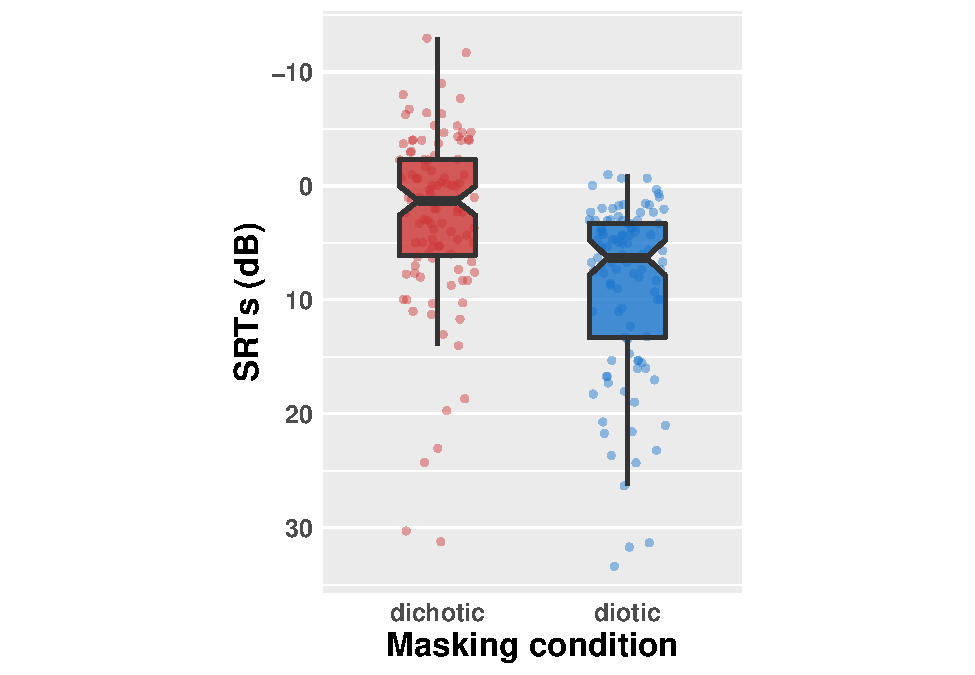
\includegraphics{results_files/figure-latex/mask-ear-fig-1.pdf}
\caption{\label{fig:mask-ear-fig}Speech recognition thresholds (SRTs) by listening condition. Smaller SRTs indicate better recognition of test material (i.e.~at more challenging signal to noise ratios). Colored points represent individual listener responses; points are horizontally jittered for readability. Boxes indicate interquartile range and whiskers 1.5 x the interquartile range in each direction. Black horizontal lines indicate the median and notches 95\% confidence intervals surrounding the median.}
\end{figure}

\begin{table}[!h]

\caption{\label{tab:srt-descrip-tbl}Descriptive statistics of SRTs (dB) by listening condition: Mean (SD) range.}
\centering
\begin{tabular}[t]{>{\raggedright\arraybackslash}p{10em}>{\raggedright\arraybackslash}p{10em}>{\raggedright\arraybackslash}p{10em}>{\raggedright\arraybackslash}p{10em}}
\toprule
Masker 
 presentation & Combined channel 
 interaction conditions & Binaural broad & L limited,
 R broad\\
\midrule
dichotic & 5.38(7.61)-8-31.2 & 9.84(7.76)0-31.2 & 0.92(4.03)-8-8.7\\
diotic & 11.11(7.99)-0.7-33.4 & 16.29(7.08)4.3-33.4 & 4.82(2.87)-0.7-11\\
\bottomrule
\end{tabular}
\end{table}

\begin{figure}
\centering
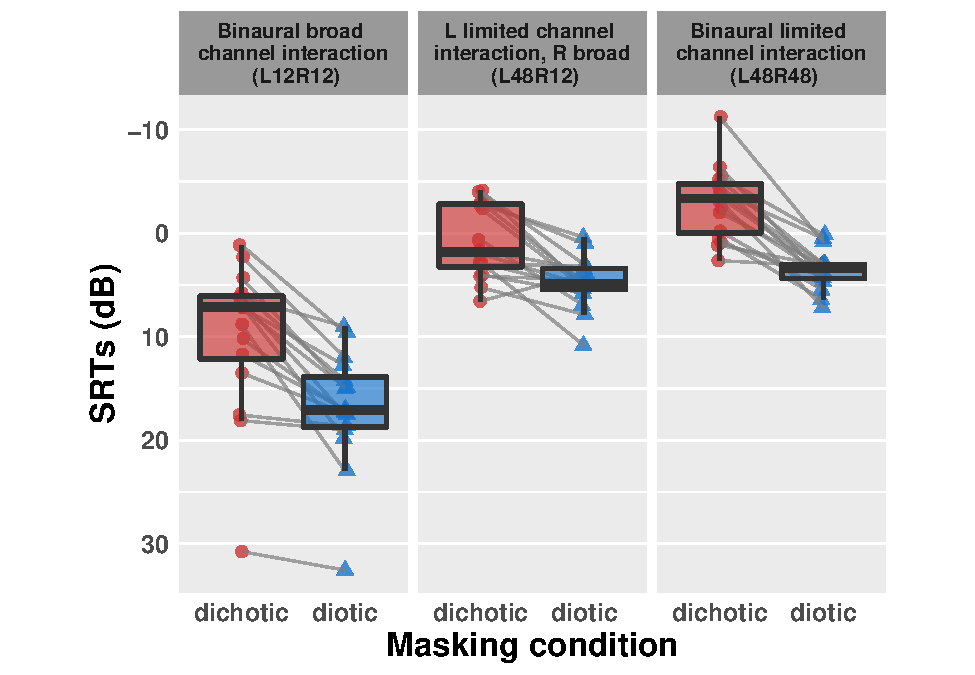
\includegraphics{results_files/figure-latex/srt-ind-1.pdf}
\caption{\label{fig:srt-ind}SRTs by channel interaction condition. Colored points represent individual listener responses; gray lines connect listener-level SRTs across masking conditions. Boxes indicate interquartile range and whiskers 1.5 x the interquartile range in each direction. Black horizontal lines indicate the median.}
\end{figure}

To complement description of these raw data, we additionally fit a linear mixed effects model to predict the effect of listening condition upon SRTs. The significance of potential model parameters was determined via comparing model log-likelihood values and AIC estimates. Categorical predictor variables were contrast-coded to assist in model interpretation. To account for individual variability and correlation stemming from participant-level effects, we included random intercepts by participant; all fixed effects were added step-wise to this baseline, random effect-only model.

Best model fit included the fixed effects of masker presentation (diotic vs.~dichotic) and channel interaction (binaural broad vs.~monaural narrow and broad), but not their interaction (see Table \ref{tab:srt-model-sum} for summary). The lack of an interaction suggests that the benefit of dichotic \textgreater{} diotic is consistent in both channel interaction conditions. Interpretation of model coefficients indicates a SRT improvement of -5.39 dB in the dichotic over diotic conditions (t=-6.8, p\textless.001) and improvement of -10.24 dB in the monaural limited-broad channel interaction over binaural broad channel interaction conditions (t=-12.87, p\textless.001). Furthermore, the significant effect of masker presentation, without an interaction, indicates significant SRM in both channel interaction conditions.

\begin{table}[!h]

\caption{\label{tab:srt-model-sum}Model predicting the effect of listening condition upon SRTs.}
\centering
\begin{tabular}[t]{lrrrrl}
\toprule
  & Est. & S.E. & t.val. & d.f. & p-value\\
\midrule
Intercept & 15.92 & 1.11 & 14.39 & 25.66 & <.001\\
Masker: dichotic & -5.39 & 0.79 & -6.80 & 127.56 & <.001\\
Channel interaction: L48R12 & -10.24 & 0.80 & -12.87 & 127.69 & <.001\\
\bottomrule
\end{tabular}
\end{table}

\hypertarget{srm-results}{%
\subsection{SRM results}\label{srm-results}}

To further evaluate the effect of masker presentation, we evaluated a second outcome variable: SRM, or the difference between the average SRT between diotic and dichotic masker conditions. Here, a higher value indicates greater release from masking or the listener benefiting more from the dichotic listening condition during listening.

As previously mentioned, significant SRM was found for both channel interaction conditions. However, the SRM was greater in the binaural broad channel interaction condition (M=6.98 (SD=4.16) than monaural L limited/R broad condition (M=3.93 (SD=3.41)) indicating greater SRM for same than different channel interaction (Figure \ref{fig:srm}).

\begin{figure}
\centering
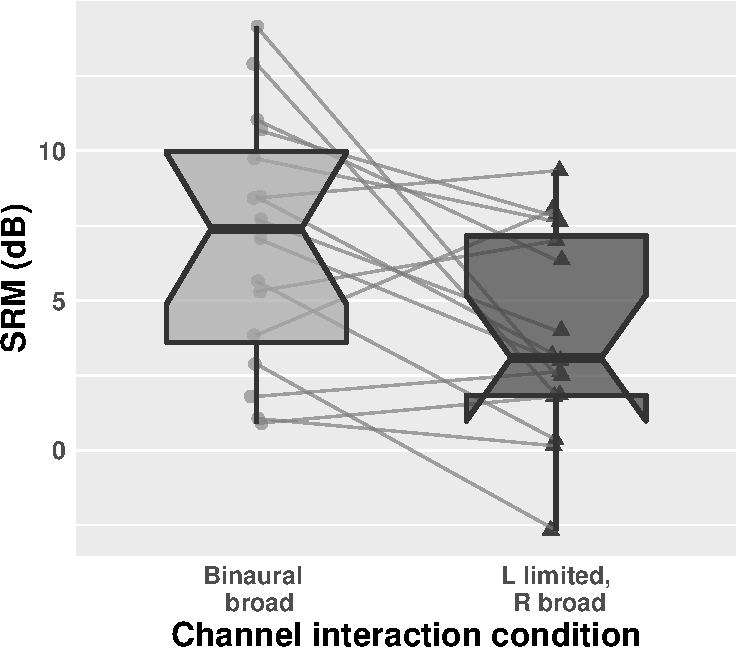
\includegraphics{results_files/figure-latex/srm-1.pdf}
\caption{\label{fig:srm}SRM (diotic-dichotic) by channel interaction condition. Higher values indicate greater benefit from dichotic over diotic listening conditions. Points represent individual listener responses; gray lines connect listener-level SRM values across channel interaction conditions. Boxes indicate interquartile range and whiskers 1.5 x the interquartile range in each direction. Black horizontal lines indicate the median and notches 95\% confidence intervals surrounding the median.}
\end{figure}

To further evaluate these results, we fit another linear mixed effects model, controlling for participant-level effects in the random effect structure (random intercepts), to predict the effect of channel interaction condition upon SRM (see Table \ref{tab:srm-model-summary} for model summary). Channel interaction condition improved upon a baseline, random effects-only model. Model coefficients show a 3.04 dB SRM benefit for the same-interaction condition (binaural broad) over the different-interaction condition (monaural broad and limited) (t=4.94, p\textless.001), suggesting that the degree of channel interaction may not interfere greatly with SRM.

\begin{table}[!h]

\caption{\label{tab:srm-model-summary}Model predicting the effect of channel interaction condition upon SRM.}
\centering
\begin{tabular}[t]{lrrrrl}
\toprule
  & Est. & S.E. & t.val. & d.f. & p-value\\
\midrule
Intercept & 3.93 & 0.84 & 4.70 & 19.9 & <.001\\
Channel interaction: L12R12 & 3.04 & 0.62 & 4.94 & 47.0 & <.001\\
\bottomrule
\end{tabular}
\end{table}

\hypertarget{extra-figures}{%
\section{Extra Figures}\label{extra-figures}}

\begin{figure}
\centering
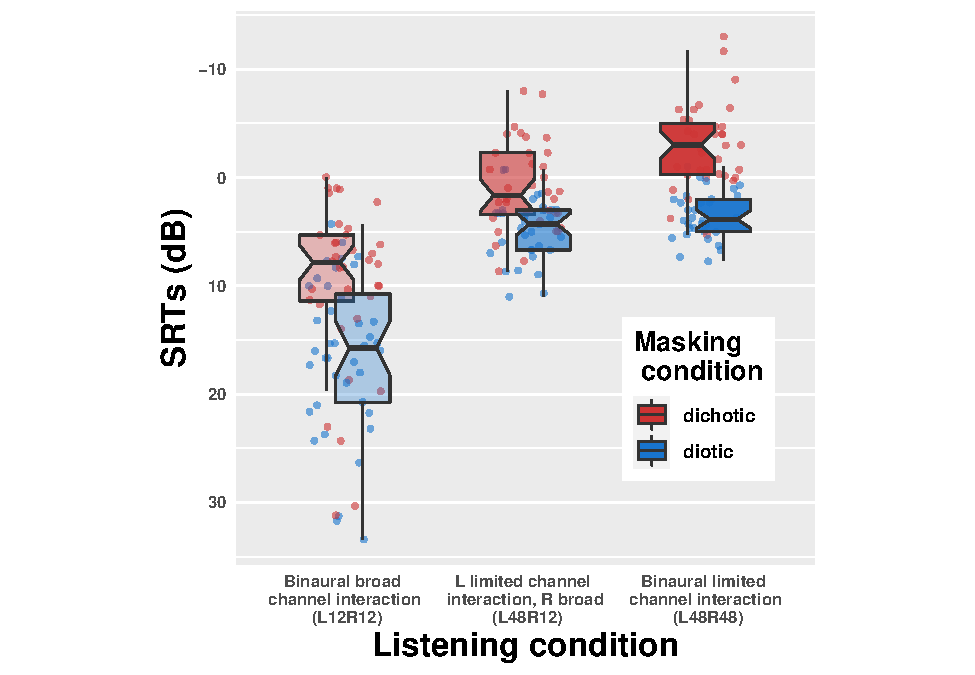
\includegraphics{results_files/figure-latex/interact-plot-1.pdf}
\caption{\label{fig:interact-plot}Speech recognition thresholds by listening condition and degree of channel interaction. Colored points represent individual listener responses; points are horizontally jittered for readability. Boxes indicate interquartile range and whiskers 1.5 x the interquartile range in each direction. Black horizontal lines indicate the median and notches 95\% confidence intervals surrounding the median.}
\end{figure}

\end{document}
